\documentclass[paper=a4, fontsize=11pt]{scrartcl} % A4 paper and 11pt font size
\usepackage{./../usfassignment}
\settitle{Assignment 7}
\setauthor{Wanzhang Sheng}
\setcourse{CS662: Artificial Inteligent}

\begin{document}

\maketitle % Print the title

% -----------------------------------------------------------------------------
% PROBLEM 1
% -----------------------------------------------------------------------------
\section{}

\begin{fancyquotes}
  (8 points) K-nearest neighbors problem:
  You are given a dataset, $D = {(x1,yes), (x2,no), (x3,yes), (x4,yes), (x5,no), (x6,yes)}$
  The values of the similarity function, $K$, for a new point $x0$ are: $K(x0,x1)=2, K(x0,x2)=1.5, K(x0,x3)=1.8, K(x0,x4)=2.3, K(x0,x5)=2.1, K(x0,x6)=1.7$
\end{fancyquotes}

\subsection{}
\begin{fancyquotes}
  What is the 1-NN classification of $x0$?
\end{fancyquotes}

$K(x0,x2)=1.5$ is the smallest one. So the 1-NN classification of $x0$
is $no$.

\subsection{}
\begin{fancyquotes}
  What is the 3-NN classification of $x0$?
\end{fancyquotes}

The three smallest similarity if $K(x0,x2)=1.5, K(x0,x6)=1.7,
K(x0,x3)=1.8$, which the classifications are $no, yes, yes$.
So the 3-NN classification of $x0$ is $yes$.

\pagebreak

% -----------------------------------------------------------------------------
% PROBLEM 2
% -----------------------------------------------------------------------------
\section{}

\begin{fancyquotes}
  (12 points) Naive Bayes

  Imagine we are building a Naive Bayes classifier to distinguish
  between two classes, $A$ and $B$.

  We have 5 documents in class $A$, containing only the following
  words with frequencies as given: money (4 times), finance (1 time),
  stock (10 times), and market (6 times).

  We have 10 documents in class $B$, containing only the following
  words with frequencies as given: money (1 time), loss (20 times),
  finance (20 times), and gain (5 times)

  Using the Naie Bayes assumption, determine whether it is more likely
  that the below document is of class A or class B. Assume that the
  conditional probability of a word given a category is its frequency
  within a category. If a word does not occur in a given category,
  assume its conditional probability is 1/10,000. Show and explain
  your work and any assumptions you make:

  Document: ``money finance loss stock gain average''
\end{fancyquotes}

$$P(A) = 5/15$$
$$P(B) = 10/15$$

$$P(\text{money}|A) = 4/21$$
$$P(\text{finance}|A) = 1/21$$
$$P(\text{stock}|A) = 10/21$$
$$P(\text{market}|A) = 6/21$$

$$P(\text{money}|B) = 1/46$$
$$P(\text{loss}|B) = 20/46$$
$$P(\text{finance}|B) = 20/46$$
$$P(\text{gain}|B) = 5/46$$

\begin{equation*}
  \begin{split}
    v_A &= P(A)\times P(\text{money}|A)\times P(\text{finance}|A)\times
    P(\text{loss}|A)\times P(\text{stock}|A)\times P(\text{gain}|A)\times
    P(\text{average}|A)\\
    &= 5/15*4/21*1/21*1/10000*10/21*1/10000*1/10000\\
    &= 1.4397293*10^{-15}
  \end{split}
\end{equation*}

\begin{equation*}
  \begin{split}
    v_B &= P(B)\times P(\text{money}|B)\times P(\text{finance}|B)\times
    P(\text{loss}|B)\times P(\text{stock}|B)\times P(\text{gain}|B)\times
    P(\text{average}|B)\\
    &= 10/15*1/46*20/46*20/46*1/10000*5/46*1/10000\\
    &= 2.9778815*10^{-12}
  \end{split}
\end{equation*}

So it's class $B$.

\pagebreak

% -----------------------------------------------------------------------------
% PROBLEM 3
% -----------------------------------------------------------------------------
\section{}

\begin{fancyquotes}
  Sentiment analysis
\end{fancyquotes}

\begin{table}[hp]
  \centering
  \begin{tabular}[hp]{ccc}
    & Pros & Cons \\
    Positive & 50.23\% & 11.26\% \\
    Negative & 49.77\% & 88.74\%
  \end{tabular}
  \caption{Without handling the negation words}
\end{table}

\begin{table}[hp]
  \centering
  \begin{tabular}[hp]{ccc}
    & Pros & Cons \\
    Positive & 50.27\% & 9.35\% \\
    Negative & 49.73\% & 90.65\%
  \end{tabular}
  \caption{With handling the negation words}
\end{table}

Not much improvement by handling the negation words.

\pagebreak


% -----------------------------------------------------------------------------
% PROBLEM 4
% -----------------------------------------------------------------------------
\section{}

\subsection{}
\begin{fancyquotes}
  (8 pts) Assume we have two classifiers, $C1$, and $C2$ for filtering
  spam. $C1$ correctly classifies spam $85\%$ of the time, but
  classifies ham as spam $8\%$ of the time. $C2$ correctly classifies
  spam $70\%$ of the time, but classifies ham as spam $2\%$ of the
  time. Assume we have $1000$ emails to process. If it costs us
  $\$0.05$ each time a spam is misclassified as ham, and $\$1$ each
  time a ham is misclassified as spam, what are the costs of using
  $C1$ and $C2$?
\end{fancyquotes}

\[\text{cost}_{c_1}
= 500\times(100\%-85\%)\times 0.05 + 500\times 8\%\times 1
= \$43.75\]
\[\text{cost}_{c_2}
= 500\times(100\%-70\%)\times 0.05 + 500\times 2\%\times 1
= \$17.5\]

$C_2$ is better.

\subsection{}
\begin{fancyquotes}
  (8 pts) Given the following information, what is the value of
  knowing whether we are in good or bad economic conditions?
  \begin{itemize}
  \item The value (utility) of buying an apartment building in good
    economic conditions is $\$50,000$ and $\$30,000$ in bad conditions
  \item The value of buying an office building in good economic
    conditions is $\$100,000$ and $-\$40,000$ in bad conditions
  \item The value of buying a warehouse in good economic conditions is
    $\$30,000$ and $\$10,000$ in bad conditions
  \item The probability of being in good economic conditions is $0.6$
    and the probability of being in bad economic conditions is $0.4$
  \end{itemize}
\end{fancyquotes}

The expectation value of buying an apartment building is
$50000*0.6+30000*0.4=42000$.
The expectation value of buying an office building is
$100000*0.6-40000*0.4=44000$.
The expectation value of buying an warehouse is
$30000*0.6+10000*0.4=22000$.

When we don't know the economic condition, we will choose buying an
office building for the most utility $44000$.

When we know the economic condition is good, we will choose buying an
office building for the most utility $100000$;
When we know the economic condition is bad, we will choose buying an
apartment building for the most utility $30000$;

So when we know the economic condition, the expected utility is
$100000*0.6+30000*0.4=72000$.

So the value of the information is $72000-44000=\$28000$.

\pagebreak

% -----------------------------------------------------------------------------
% PROBLEM 5
% -----------------------------------------------------------------------------
\section{}

\subsection{}
\begin{fancyquotes}
  (6 pts) For the $4\times3$ world shown in Fig~\ref{fig:mdp} of R\&N,
  calculate which squares can be reached by the action sequence [Up,
  Up, Right, Right, Right] and with what probabilities.
\end{fancyquotes}

\begin{figure}[hp]
  \centering
  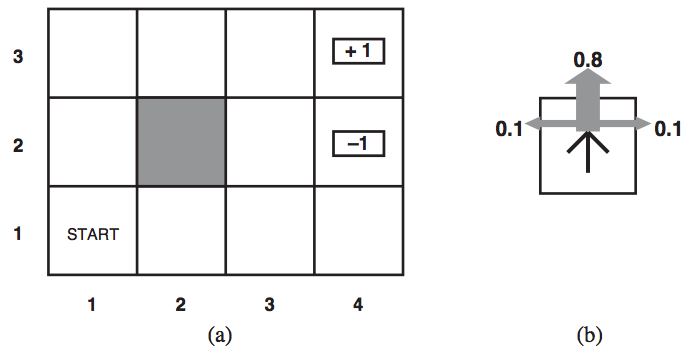
\includegraphics[width=\textwidth]{mdp.png}
  \caption{MDP}
\label{fig:mdp}
\end{figure}

\begin{table}[hp]
  \centering
  \begin{tabular}[hp]{crrrr}
    3 & 0.02524 & 0.06224 & 0.17994 & 0.32792 \\
    2 & 0.18054 & 0.0 & 0.04443 & 0.01368 \\
    1 & 0.02462 & 0.02824 & 0.02627 & 0.08688 \\
    & 1 & 2 & 3 & 4
  \end{tabular}
  \caption{MDP probabilities}
\label{tab:mdp}
\end{table}

\pagebreak

\subsection{}
\begin{fancyquotes}
  (9 pts) Below is a set of utilities for states in our simple grid
  world. Show the calculation that the value iteration algorithm would
  make for square $3$. What is the updated utility? Show all your
  work.
\end{fancyquotes}

\begin{figure}[hp]
  \centering
  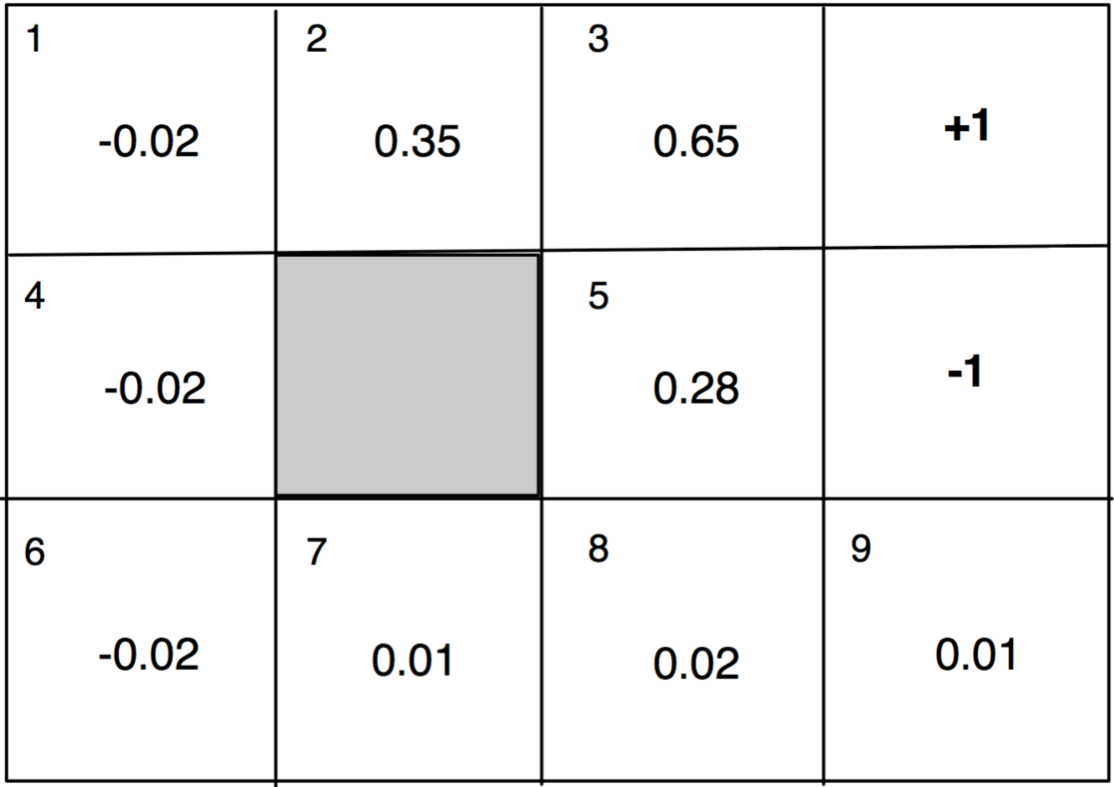
\includegraphics[width=0.7\textwidth]{mdp_utility.png}
  \caption{MDP}
\label{fig:mdpu}
\end{figure}

$$U(s) = R(s) + \gamma\max_a(\Sigma P(t|s,a)U(t))$$
\[
\begin{split}
  U(3) = -0.04 + \gamma\max(& 0.8U(3)+0.1U(2)+0.1U(+1),\\
  & 0.8U(+1)+0.1U(3)+0.1U(5),\\
  & 0.8U(5)+0.1U(+1)+0.1U(2),\\
  & 0.8U(2)+0.1U(5)+0.1U(3))\\
\end{split}
\]
$$U(3) = -0.04 + \gamma\max(0.655, 0.893, 0.359, 0.373)$$
$$U(3) = -0.04 + 0.8 * 0.893$$
$$U(3) = 0.6744$$

\pagebreak

\end{document}